\documentclass[11pt]{article}
\usepackage{amsmath, amssymb, amsfonts,  graphicx, enumerate, float}
\usepackage[margin=0.5in]{geometry}
\graphicspath{{./}}
\newcommand*{\vs}{\vspace{1cm}}
\newcommand*{\next}{\noindent}
\newcommand*{\set}{\setcounter{equation}{1}}



\title{3.2 Rolle's Theorem and the Mean Value Theorem}
\author{Juan J. Moreno Santos}
\date{October 2023}

\begin{document}

\maketitle

\section{Explain why Rolle's Theorem does not apply to the function even though there exist $a$ and $b$ such that $f(a)=f(b)$.}
2.\[f(x)=\cot\frac{x}{2},\,\,\,[\pi, 3\pi]\]
Rolle's Theorem does not apply because $f$ is not continuous at $x=2\pi$.

\vs
\next
4.\begin{eqnarray}
    f(x)=\sqrt[]{(2-x^{2/3})}\\
    f(-1)=1=f(1)\\
    f'(x)=\frac{-\,\,\sqrt[]{(2-x^{2/3})^3}}{x^{1/3}}
\end{eqnarray}
Rolle's Theorem does not apply because $f$ is not differentiable at $x=0$

\section{Find the two x-intercepts of the function $f$ and show that $f'(x)=0$ at some point between the two x-intercepts.}
6.\[f(x)=x(x-3)\]
(0,0) and (3, 0) are x-intercepts
\[f'(x)=2x-3=0\,\,\,\,\,\,\text{at}\,\,\,\,\,\,x=\frac{3}{2}\]

\vspace{1cm}
\noindent
8.\[f(x)=-3x\,\,\sqrt[]{x+1}\]
(-1, 0) and (0, 0) are x-intercepts
\begin{eqnarray}
    \setcounter{equation}{1}
    f'(x)&=-3x\frac{1}{2}(x+1)^{-1/2}-3(x+1)^{1/2}\\
    &=-3x(x+1)^{-1/2}\left(\frac{x}{2}+(x+1)\right)\\
    &=-3(x+1)^{-1/2}\left(\frac{3}{2}x+1\right)\,\,\,\,\text{at}\,\,\,\, x=\frac{2}{3}
\end{eqnarray}

\section{The graph of $f$ is shown. Apply Rolle's Theorem and find all values of $c$ such that $f'(c)=0$ at some point between the labeled intercepts.}
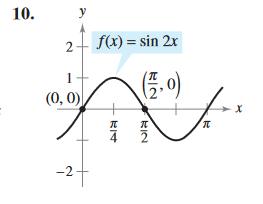
\includegraphics{10.png}\\
\begin{eqnarray}
    \setcounter{equation}{1}
    f(x)&=\sin2x\\
    f(0)&=f\left(\frac{\pi}{2}\right)=0\\
    f'(x)&=2\cos2x=0\,\,\,\,\text{at}\,\,\,\, x=\frac{\pi}{4}
\end{eqnarray}

\section{Determine whether Rolle's Theorem can be applied. If Rolle's Theorem can be applied, find all values of $c$ in the open interval $(a, b)$ such that $f'(c)=0$. If Rolle's Theorem cannot be applied, explain why not.}
12.\begin{eqnarray}
    \setcounter{equation}{1}
    f(x)&=x^2-5x+4,\,\,\,\,[1, 4]\\
    f(1)&=0=f(4)\\
\end{eqnarray}
Rolle's Theorem applies since $f$ is continuous on $[1, 4]$ and differentiable on (1, 4).
\begin{eqnarray}
    f'(x)&=2x-5\\
    &2x-5=0\therefore x=\frac{5}{2}=c
\end{eqnarray}

\vspace{1cm}
\noindent
14.\begin{eqnarray}
    \setcounter{equation}{1}
    f(x)&=(x-3)(x+1)^2,\,\,\,\,[1, 3]\\
    f(-1)&=f(3)=0
\end{eqnarray}
Rolle's Theorem applies since $f$ is continuous on [1, 3] and differentiable on (-1, 3).
\begin{eqnarray}
    f'(x)&=(2)(x-3)(x+1)+(x+1)^2\\
    &=(x+1)(2x-6+x+1)\\
    &=(x+1)(3x-5)\therefore c=\frac{5}{3}
\end{eqnarray}

\vspace{1cm}
\noindent
18.\begin{eqnarray}
    \setcounter{equation}{1}
    f(x)=\frac{x^2-1}{x},\,\,\,\,[-1, 3]
    f(-1)=0=f(1)
\end{eqnarray}
Rolle's Theorem doesn't apply since $f$ is not continuous on [-1, 1] because $f(0)$ is undefined.

\vspace{1cm}
\noindent
22.\begin{eqnarray}
\setcounter{equation}{1}
    f(x)=\cos2x,\,\,\,\,[-\pi, \pi]
    f(-pi)=1=f(\pi)
\end{eqnarray}
Rolle's Theorem applies since $f$ is continuous on $[-\pi, \pi]$ and differentiable on $(-\pi, \pi)$.
\begin{eqnarray}
    f'(x)&=-2\sin2x\\
    -2\sin2x&=0\\
    \sin2x&=0\therefore x=-\pi, -\frac{\pi}{2}, 0, \frac{\pi}{2}, \pi\\
    c&=-\frac{\pi}{2}, 0, \frac{\pi}{2}\\
\end{eqnarray}

\section{Determine whether Rolle's Theorem can be applied to $f$ on the interval and, if so, find all values of $c$ in the open interval $(a, b)$ such that $f'(c)=0$}
26.\begin{eqnarray}
    \setcounter{equation}{1}
    f(x)=x-x^{1/3},\,\,\,\,[0, 1]
    f(0)=0=f(1)
\end{eqnarray}
Rolle's theorem applies since $f$ is continuous on [0, 1] and differentiable on (0, 1)
\begin{eqnarray}
    f'(x)&=1-\frac{1}{3\sqrt[3]{x^2}}=0\\
    1&=\frac{1}{3\sqrt[3]{x^2}}\\
    \sqrt[3]{x^2}&=\frac{1}{3}\\
    x^2&=\frac{1}{27}\\
    x&=\sqrt[]{\frac{1}{27}}=\frac{\sqrt[]{3}}{9}=c
\end{eqnarray}

\section{Copy the gaph and sketch the secant line to the graph through the points $(a, f(a))$ and $(b, f(b))$. Then sketch any  tangent lines to the graph for each value of $c$ guaranteed by the Mean Value Theorem.}
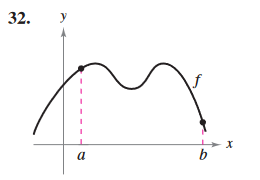
\includegraphics[scale=1]{32a.png}
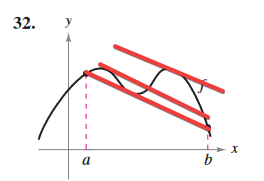
\includegraphics[scale=1]{32b.png}

\section{Explain why the Mean Value Theorem does not apply to the function $f$ on the interval $[0, 6]$}
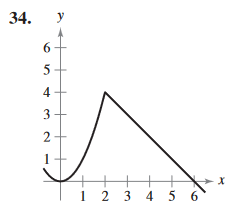
\includegraphics{34.png}
The Mean Value Theorem doesn't apply since f is not differentiable at $x=2$.

\section{Determine whether the Mean Value Theorem can be applied to $f$ on the closed interval $[a, b]$. If the Mean Value Theorem can be applied, find all values of $c$ in the open interval $(a, b)$ such that $f'(c)=\frac{f(b)-f(a)}{b-a}$. If the Mean Value Theorem cannot be applied, explain why not.}
42.\[f(x)=x^4=8x,\,\,\,\,[0, 2]\]
The function is differentiable on (0, 2) and continuous on [0, 2].
\begin{eqnarray}
    \setcounter{equation}{1}\\
    \frac{f(2)-f(0)}{2-0}&=\frac{0}{2}=0\\
    f'(x)&=4x^3-8=4(x^3-2)=0\\
    x^3&=2\\
    x&=\sqrt[3]{2}=c
\end{eqnarray}

\vspace{1cm}
\noindent
44.\[f(x)=\frac{x+1}{x},\,\,\,\,[-1, 2]\]
The Mean Value Theorem doesn't apply because $f(x)$ is not continuous at $x=0$.

\vspace{1cm}
\noindent
48.\[f(x)=\cos x+\tan x,\,\,\,\,[0, \pi]\]
The Mean Value Theorem doesn't apply because $f(x)$ is not continuous at $x=\frac{pi}{2}$.

\section{(a) Graph the function $f$ on the given interval, (b) find and graph the secant line through the points on the graph of $f$ at the endpoints of the given interval, and (c) find and graph any tangent lines to the graph of $f$ that are parallel to the secant line.}
52.\[f(x)=x^4-2x^3+x^2,\,\,\,\,[0, 6]\]\\
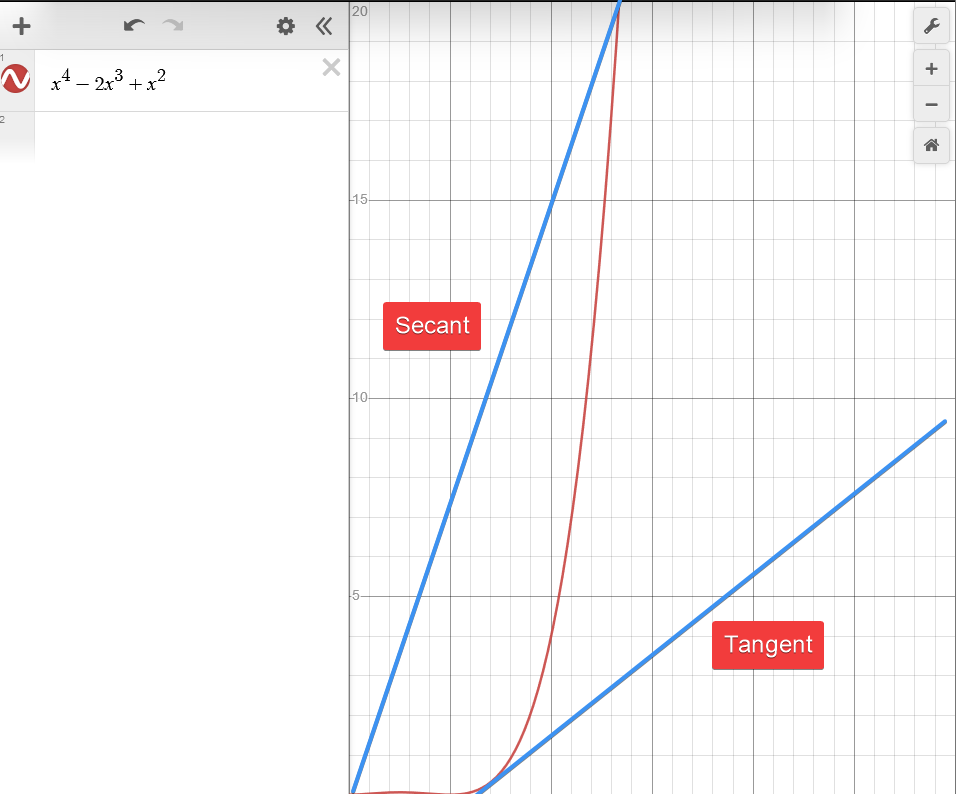
\includegraphics[scale=0.5]{52.png}\\

\section{Word problems}
54. A company introduces a new product for which the number of units sold $S$ is \[S(t)=200\left(5-\frac{9}{2+t}\right)\] where $t$ is the time in months.\\
(a) Find the average rate of change of $S(t)$ during the first year.
\begin{eqnarray}
    \setcounter{equation}{1}
    \frac{S(12)-S(0)}{12-0}=\frac{200(5-\frac{9}{14}-200(5-\frac{9}{2}))}{12}=\frac{450}{7}
\end{eqnarray}
(b) During what month of the first year does $S'(t)$ equal the average rate of change?
\begin{eqnarray}
    S'(t)&=200\left(\frac{9}{(2+t)^2}\right)=\frac{450}{7}\\
    \frac{1}{(2+t)^2}&=\frac{1}{28}\\
    2+t&=2\sqrt[]{7}\\
    t&=2\,\,\sqrt[]{7}-2\approx 3.3 \text{months}
\end{eqnarray}

\vspace{1cm}
\noindent
60. When an object is removed from a furnace and placed in an environment with a constant temperature of 90°F, its core temperature is 1500°F. Five hours later the core temperature is 390°F. Explain why there must exist a time in the interval when the temperature is decreasing at a rate of 222°F per hour.
Let $F(t)$ be the object's temperature.
\begin{eqnarray}
    \setcounter{equation}{1}
    F(0)=1500 and F(5)=390
\end{eqnarray}
The average temperature over [0, 5] is
\begin{eqnarray}
    \frac{390-1500}{5}=-222\text{°}F/h
\end{eqnarray}
As per the Mean Value Theorem, the exists a time $t_0$ such that $F'(t_0)=-222\text{°}F/h,\,\,\,\,0<t_0<5$.

\vspace{1cm}
\noindent
62. At 9:13AM, a sports car is traveling 35 miles per hour. Two minutes later, the car is traveling 85 miles per hour. Prove that at some time during this two-minute interval, the car's acceleration is exactly 1500 miles per hour squared.\\
Let $t=0$ be 9:13AM. As per the Mean Value Theorem, there exists a $t_0$ in $(0, \frac{1}{30})$ such that
\[v'(t_0)=a(t_0)=\frac{85-35}{\frac{1}{30}}=1500\text{mi/h$^2$}\]

\section{Capstone}
64. The figure shows two parts of the graph of a continuous differentiable function $f$ on [-10, 4]. The derivative of $f'$ is also continuous.\\
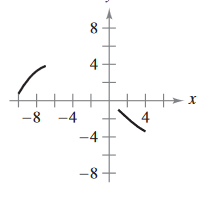
\includegraphics{64.png}\\
(a) Explain why $f$ must have at least one zero in [-10, 4]
\[f(-8)>0, f(3)<0\]
$f$ is continuous and changes sign. By the Intermediate Value Theorem, there is at least one $x$ in [-10, 4] that satisfies $f(x)=0$\\

\vspace{1cm}
\noindent
(b) Explain why $f'$ must also have at least one zero in the interval [-10, 4]. What are these zeros called?
There are numbers $a$ and $b$ such that
\[f(a)=2=f(b),\,\,\,\,-10<a<b<4\]
By Rolle's Theorem, there is a least one $c$ in (-10, 4) such that $f'(c)=0$.\\
This zero is called a critical number.

\vspace{1cm}
\noindent
(c) Make a possible sketch of the function with one zero of $f'$ on the interval [-10, 4].\\
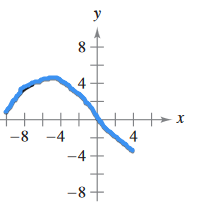
\includegraphics{64b.png}

\vspace{1cm}
\noindent
(d) Make a possible sketch of the function with two zeros of $f'$ on the interval [-10, 4].\\
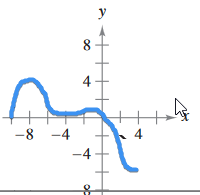
\includegraphics{64c.png}

\vspace{1cm}
\noindent
(e) Were the conditions of continuity of $f$ and $f'$ necessary to do parts (a) through (d)? Explain.\\
No. $f'$ could have been discontinous on [-10, 4].

\section{Determine whether the statement is true or flase. If it is false, explain why or give an example that shows it is false.}
77. The Mean Value Theorem can be applied to $f(x)=\frac{1}{x}$ on the interval [-1, 1].\\
\indent False. $f(x)$ is discontinous at $x=0$.

\vspace{1cm}
\noindent
78. If the graph of a function has three x-intercepts, then it must have at least two points at which its tangent line is horizontal.\\
\indent False. $f$ also has to be continuous and differentiable on each interval. For example, $f(x)=\frac{x^3-4x}{x^2-1}$.

\vspace{1cm}
\noindent
79. If the graph of a polynomial function has three x-intercepts, then it must have at least two points at which its tangent line is horizontal.\\
\indent True.

\vspace{1cm}
\noindent
80. If $f'(x)=0$ for all $x$ in the domain of $f$, then $f$ is a constant function.\\
\indent True.
\end{document}